\section*{Тестирование}
\addcontentsline{toc}{section}{Тестирование}

Тестирование выполнялось путем проверки работоспособности приложения на каждом этапе его использования.

Так как в проекте предусмотрено два различных и параллельных друг другу способа взаимодействия с приложением,
ниже будет рассмотрен каждый из них. Для удобства работа с приложением командной строки будет приведена
в листингах, а с веб-версией -- снимками экрана. Причем в листингах знаком ">" будет обозначаться введенная
bash-команда.

В качестве примера будет рассмотрен курс <<Базы данных>>, преподаваемый на кафедре <<Теоретическая информатика и компьютерные технологии>>
Вишняковым Игорем Эдуардовичем.

Первым делом необходимо создать кафедру, на которой работает пользователь.

Необходимые действия, которые нужно сделать в приложении командной строки, приведены в листинге ~\ref{cli_add_department}.

\begin{lstlisting}[language=bash, caption = {Добавление кафедры}, captionpos=b, label={cli_add_department}]
> cli department prototype
Open department.txt and fill prototype struct with 
correct data
> nano department.txt 
> cli department add
\end{lstlisting}

В файле department.txt будет находиться JSON-объект, для которого будет необходимо заполнить поле \texttt{title}
необходимым значением.

В случае работы с веб-приложением нужно выбрать необходимую таблицу, после чего в нее автоматически загрузится прототип
искомой JSON-структуры, который следует модифицировать и отправить на сервер кнопкой \texttt{Upload}, расположенной справа снизу
от поля ввода текста. Иллюстрацию можно видеть на рисунке ~\ref{web_add_department}.

\begin{figure}[h!]
	\center{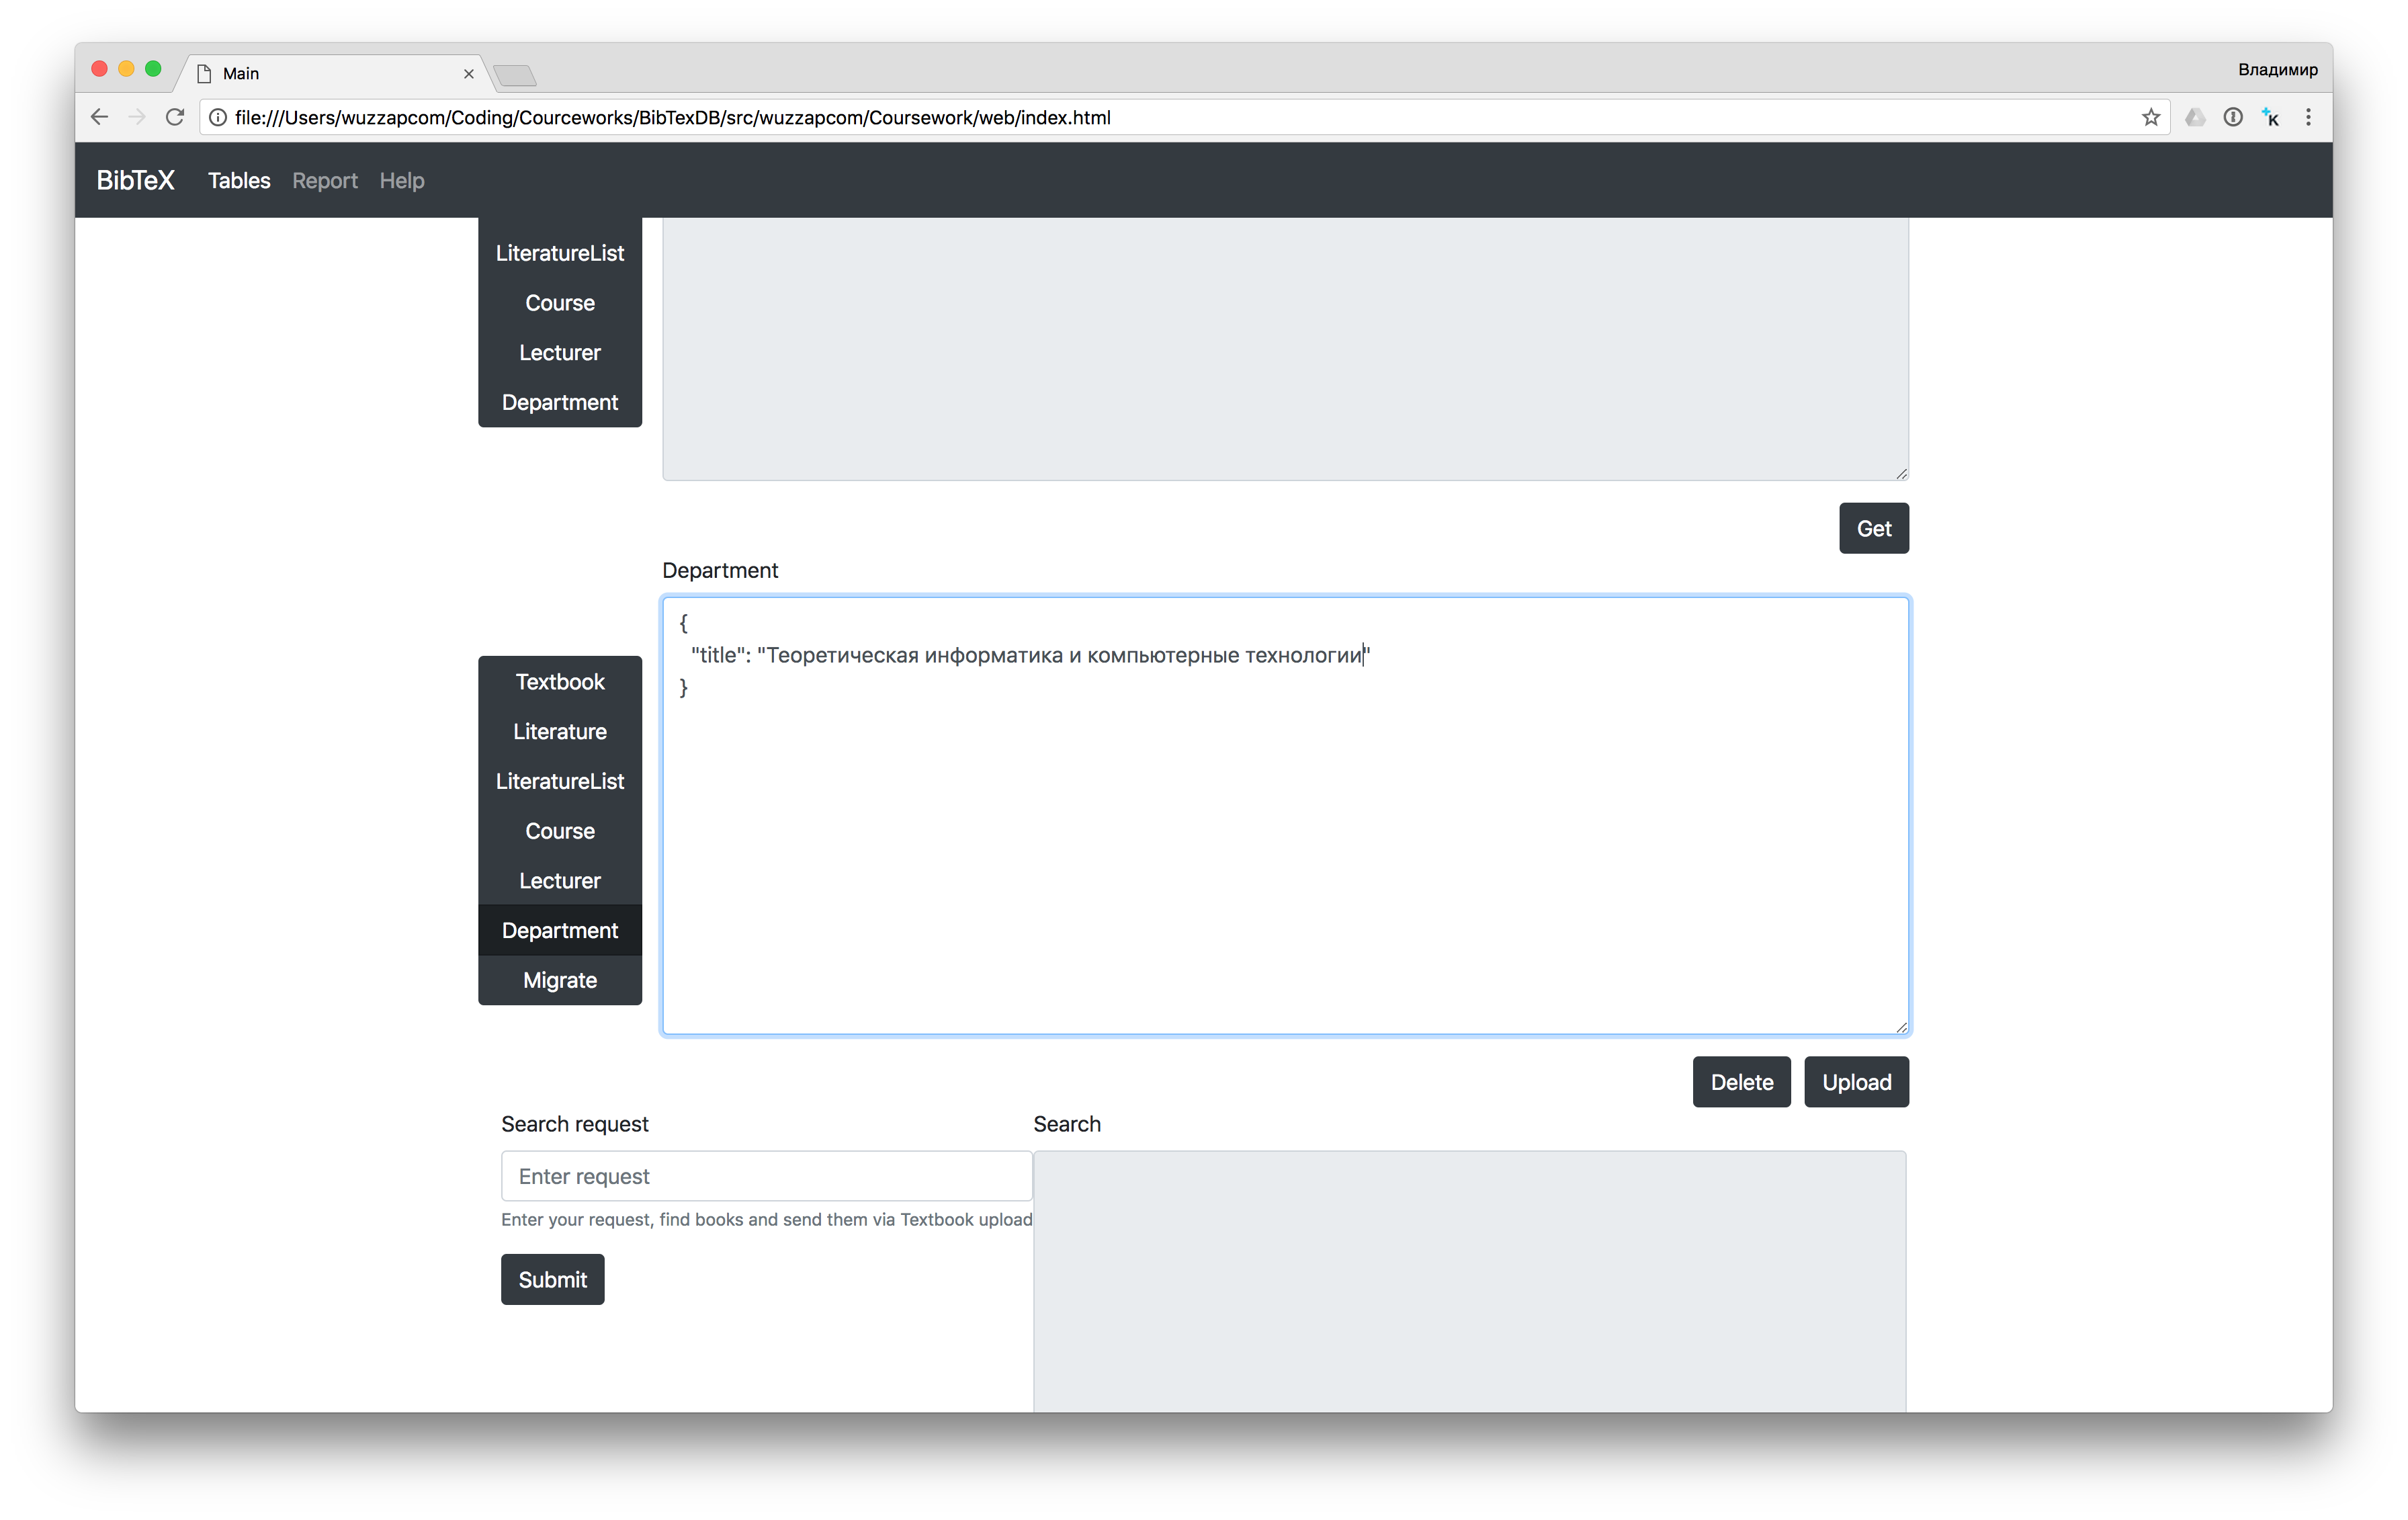
\includegraphics[width=1\linewidth]{web_add_department.png}}
	\caption{Добавление новой кафедры в веб-приложении}
	\label{web_add_department}
\end{figure}

Следующее действие -- добавление лектора к только что введенной кафедре. Последовательность действий
ничем не отличается от предыдущего шага и ее можно увидеть в листинге ~\ref{cli_add_lecturer} и рисунке
~\ref{web_add_lecturer}.

\begin{lstlisting}[language=bash, caption = {Добавление лектора}, captionpos=b, label={cli_add_lecturer}]
> cli lecturer prototype
Open lecturer.txt and fill prototype struct with correct data
> nano lecturer.txt 
> cli lecturer add
\end{lstlisting}

\begin{figure}[h!]
	\center{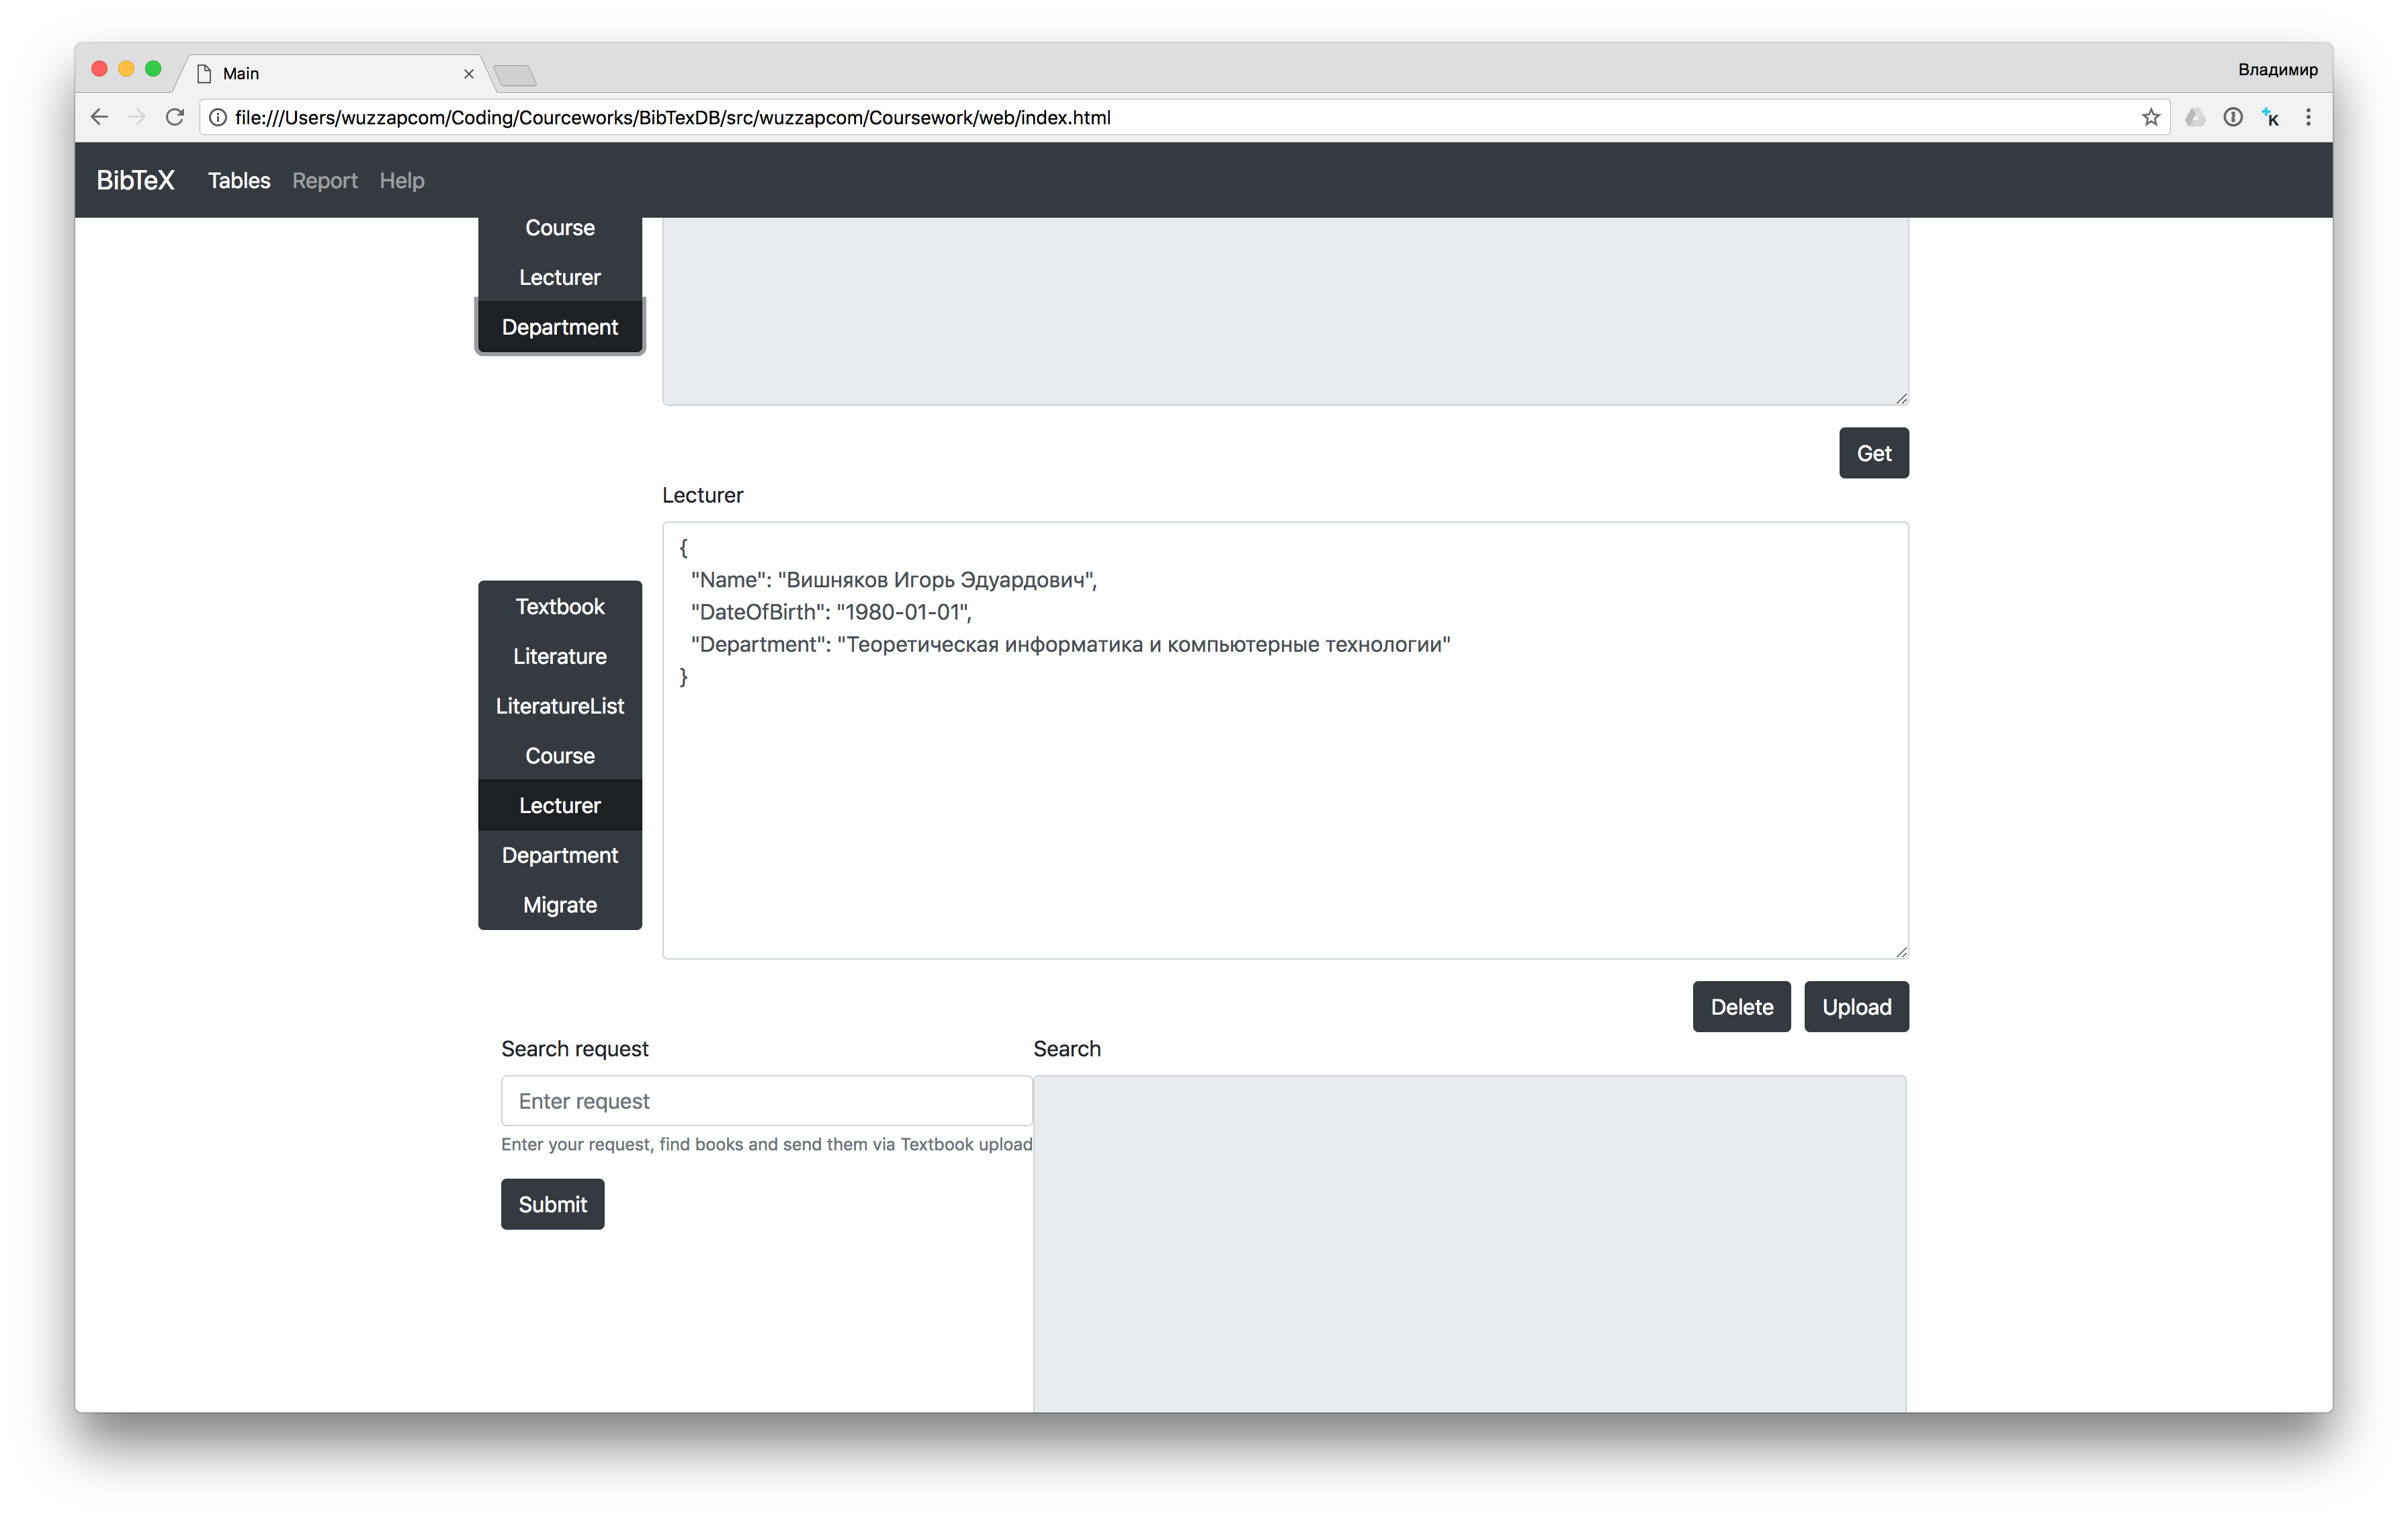
\includegraphics[width=1\linewidth]{web_add_lecturer.png}}
	\caption{Добавление нового лектора в веб-приложении}
	\label{web_add_lecturer}
\end{figure}

На шаге добавления курса становится видно преимущество веб-версии по сравнению с приложением командной строки.
Оно позволяет в двух разных окнах вводить информацию и делать запросы к базе данных. Иллюстрацию можно видеть
на рисунке ~\ref{web_add_course}. В этом примере можно держать перед глазами список добавленных лекторов чтобы,
например, не забыть дату рождения, и одновременно вводить данные об учебном курсе.

\begin{figure}[h!]
	\center{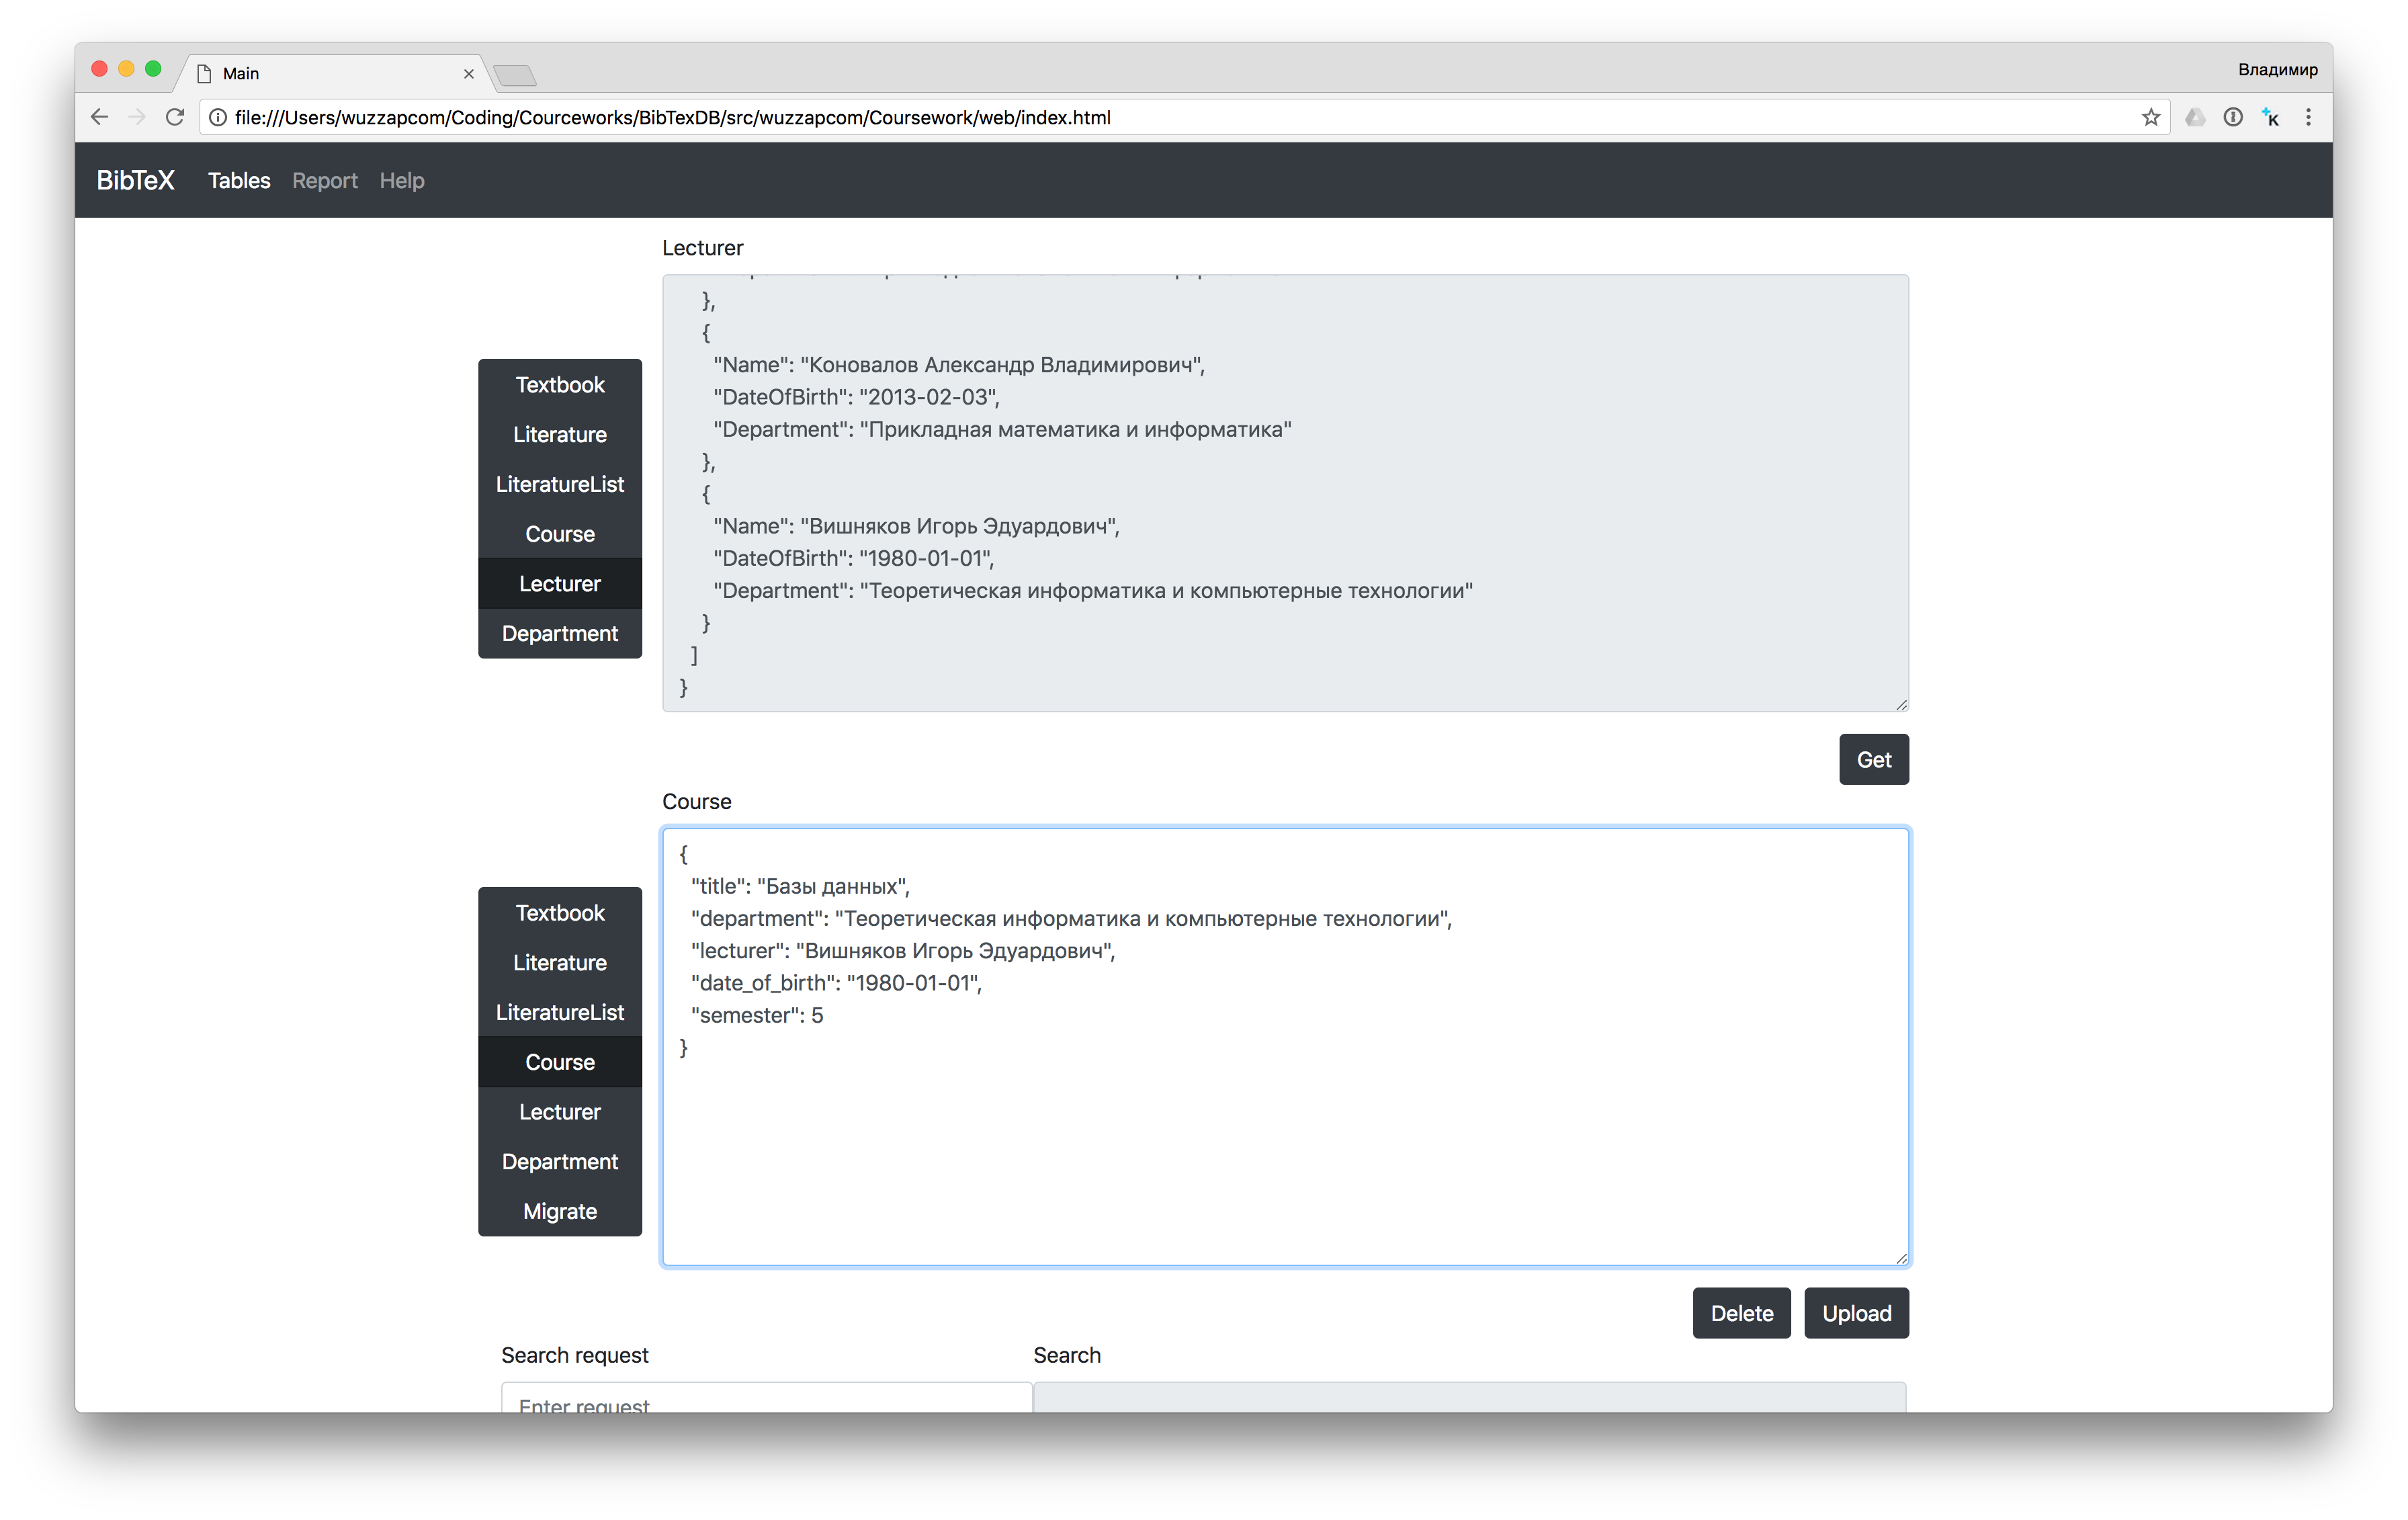
\includegraphics[width=1\linewidth]{web_add_course.png}}
	\caption{Добавление учебного курса в веб-приложении}
	\label{web_add_course}
\end{figure}

В то время как в приложении командной строки такой возможности нет. Как вариант, можно отдельно запросить список
лекторов командой \texttt{cli lector get}, чтобы открыть его в отдельном окне терминала или текстовом редакторе, но этот вариант 
явно проигрывает по удобству. Так что последовательность команд остается аналогичной и приведена в листинге ~\ref{cli_add_course}.

\begin{lstlisting}[language=bash, caption = {Добавление лектора}, captionpos=b, label={cli_add_course}]
> cli course prototype
Open course.txt and fill prototype struct with correct data
> nano course.txt 
> cli course add
\end{lstlisting}

Этап добавления нового учебного курса ничем не отличается от всех предыдущих, так что имеет смысл перейти к добавлению книг в приложение.
Как уже было сказано выше, для этого предусмотрен модуль, позволяющий использовать сервис Google Books для поиска информации о
книгах. Но возможно и добавление книг вручную, если нужного учебника не нашлось в базе сервиса. 
Для начала рассмотрим эту функцию в приложении командной строки из листинга ~\ref{cli_search}.

\begin{lstlisting}[language=bash, caption = {Поиск книг по запросу SQL в сервисе Google Books в приложении командной строки.}, captionpos=b, label={cli_search}]
> cli search --request="SQL"
Open searchResults.txt, view results, remove wrong 
items and fix incorrect data.
> nano searchResults.txt 
> cli book prototype
Open book.txt and fill prototype struct with correct data
> nano book.txt
> cli book add
\end{lstlisting}

Другими словами, необходимо сначала выполнить поиск, получить результат в файл, после чего скопировать нужную книгу в
\texttt{book.txt} и добавить ее командой \texttt{cli book add}.

Схожий принцип, но более удобный, используется и в веб-приложении, что можно увидеть на рисунке ~\ref{web_search}.

\begin{figure}[h!]
	\center{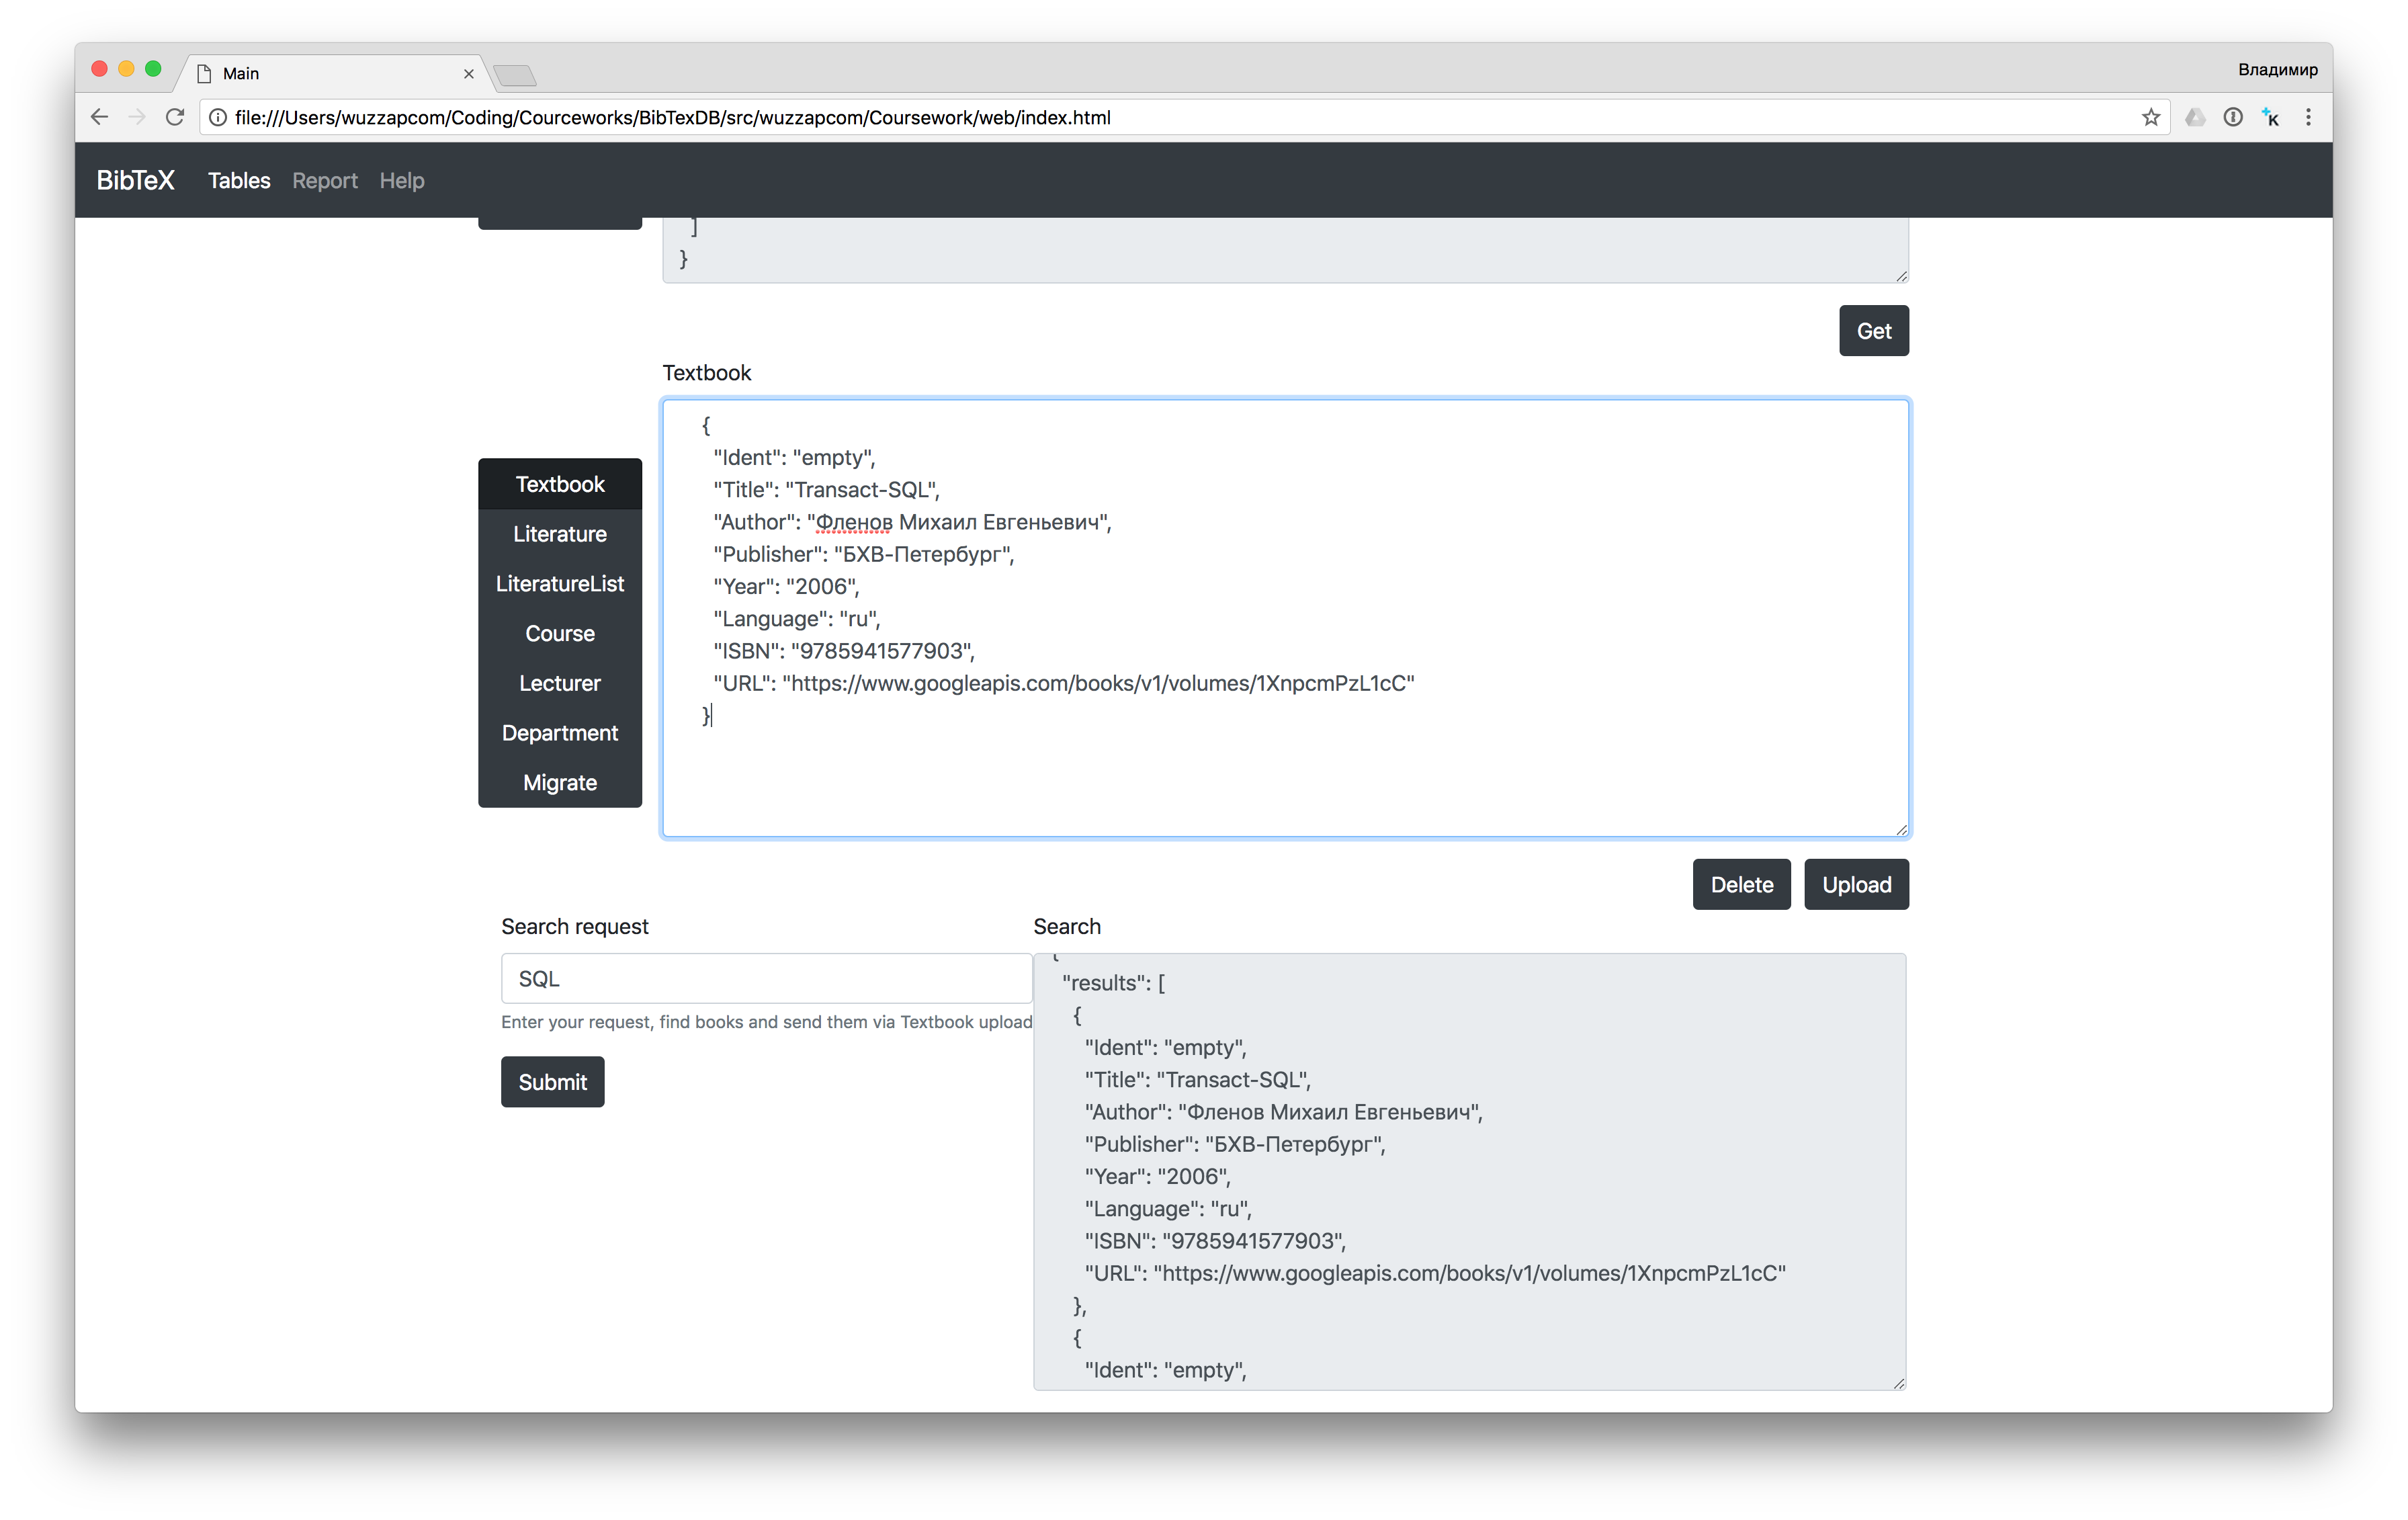
\includegraphics[width=1\linewidth]{web_search.png}}
	\caption{Поиск книг по запросу SQL в сервисе Google Books в веб-приложении.}
	\label{web_search}
\end{figure}

Добавление книги в список литературы также является набором тех же самых действий, так что имеет смысл перейти сразу к дополнительной функции:
миграции списков литературы. По своей сути, эта функция является абсолютно тем же заполнением нужной JSON-структуры, так что будет
удобно привести только вариант веб-приложения. Его можно видеть на рисунке ~\ref{web_migrate}.

\begin{figure}[h!]
	\center{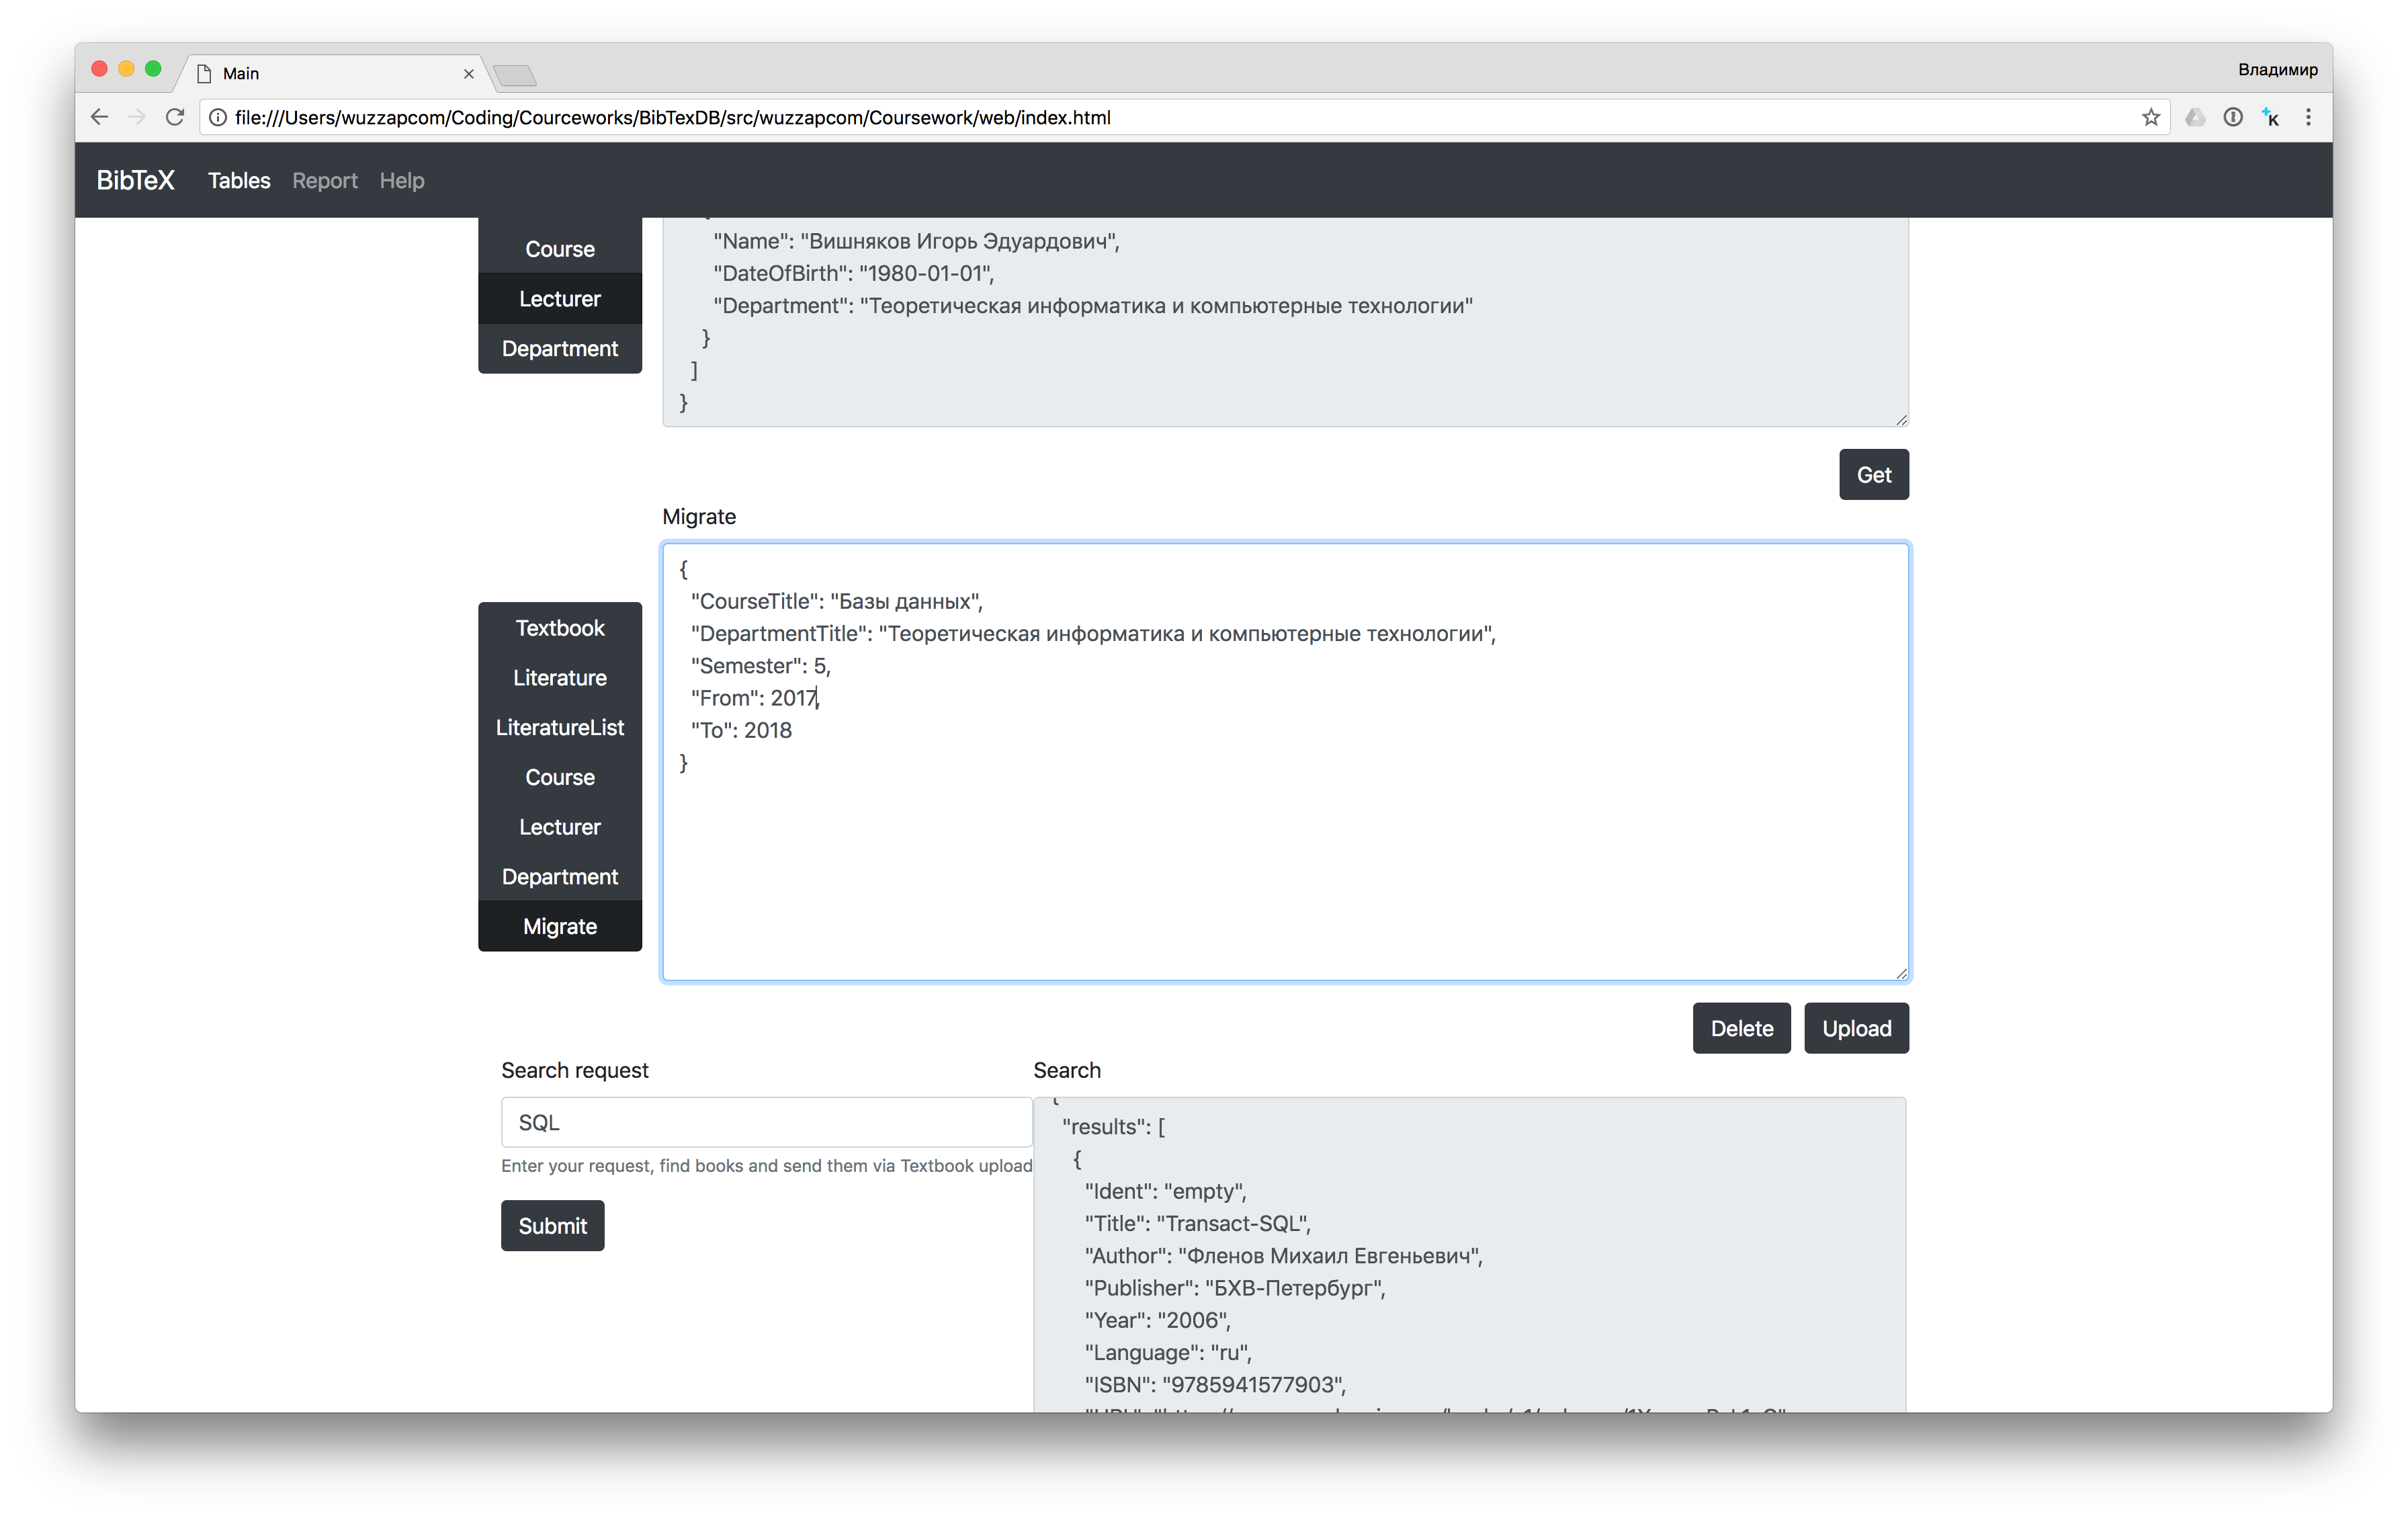
\includegraphics[width=1\linewidth]{web_migrate.png}}
	\caption{Демонстрация миграции списка литературы в веб-приложении.}
	\label{web_migrate}
\end{figure}

Важной деталью, которую необходимо отметить и зафиксировать, является то, что необходимо создать заранее тот список литературы, в который
будет производиться миграция.

Наконец стало возможным перейти к основному и самому важному пункту -- генерации самого отчета.

Для начала рассмотрим, как происходит генерация в приложении командной строки. Запрос необходимого отчета
происходит через отправку на сервер нужного списка литературы. Таким образом, запросить отчет можно последовательностью
команд из листинга ~\ref{cli_report}.

\begin{lstlisting}[language=bash, caption = {Запрос отчета в приложении командной строки.}, captionpos=b, label={cli_report}]
> cli literatureList prototype
Open literatureList.txt and fill prototype struct 
with correct data
> nano literatureList.txt
> cli report --outputFile="report.bib"
\end{lstlisting}

Как можно видеть, в команде \texttt{cli report} явным образом указан файл, в который будет записан результат. В случае
отсутствия этого флага отчет будет выведен в стандартный поток вывода, о чем сказано в справке данной команды.

Намного более удобно устроен весь процесс в веб-приложении. Специально для этого в нем сделано отдельное окно \texttt{Report}.
В нем отображаются все списки литературы, по нажатию на которые браузером сохраняется текстовый файл \texttt{report.bib}.
Рисунок ~\ref{web_report} демонстрирует данную функцию.

\begin{figure}[h!]
	\center{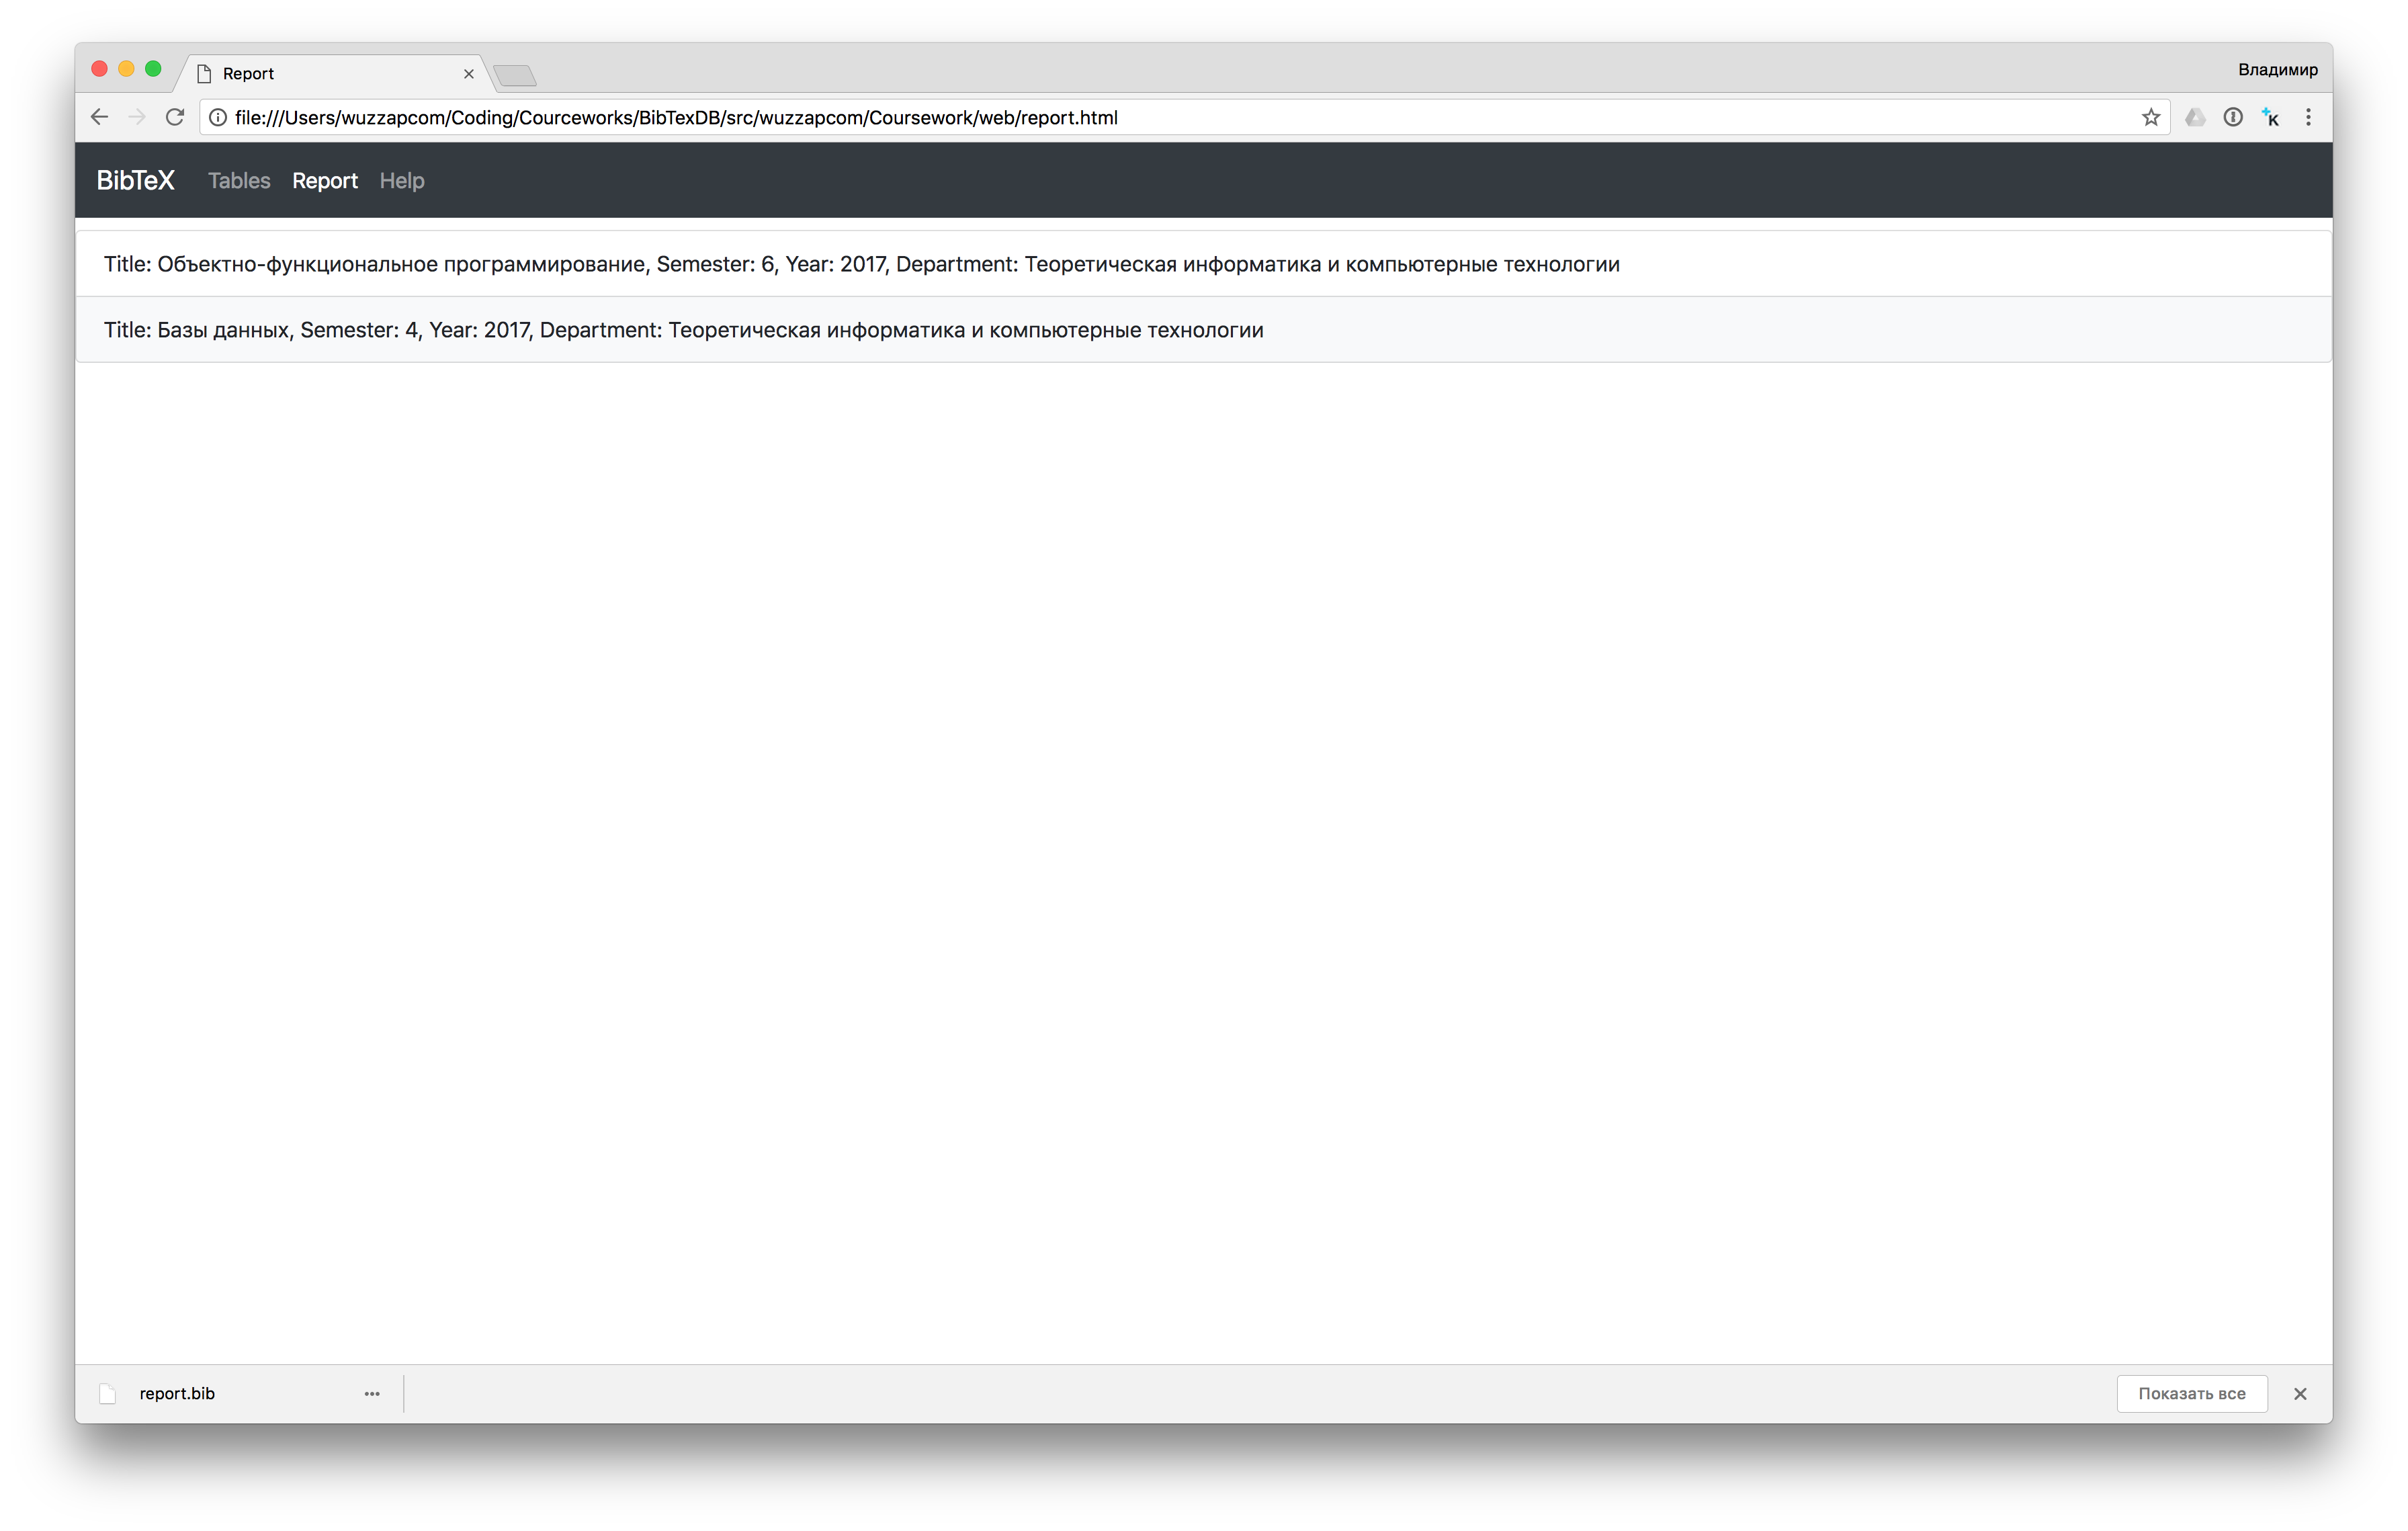
\includegraphics[width=1\linewidth]{web_report.png}}
	\caption{Демонстрация генерации отчета в веб-приложении.}
	\label{web_report}
\end{figure}

В качестве заключения хочется отметить, что работоспособность веб-приложения была проверена в браузерах Safari и Chrome на ноутбуке
под управлением операционной системы MacOS.

Таким образом, в данном разделе был рассмотрен полный цикл использования разработанного приложения, а также был продемонстрирован
принцип работы двух клиентских программ: веб-сайта и приложения командной строки. По результатам данного тестирования можно сказать, что
приложение командной строки выигрывает в автоматизируемости, но является неудобным при использовании человеком, в то время как 
веб-сайт, наоборот, предоставляет пользователю дополнительные функции для улучшения качества работы с разработанным приложением.
